\documentclass[aspectratio=169]{beamer}

\usepackage{xltxtra}
\usepackage[english, russian]{babel}[2014/03/24]% Языки: русский, английский
\setmainfont{Arial}
\setromanfont{Times New Roman}
\setsansfont{Arial}
\setmonofont{Courier New}

% Библиография
\usepackage[backend=biber, style=numeric, sorting=none]{biblatex}
\addbibresource{../../../biblio/author.bib}
\addbibresource{../../../biblio/external.bib}

%%% Таблицы %%%
\usepackage{longtable} % Длинные таблицы
\usepackage{multirow,makecell}   % Улучшенное форматирование таблиц
\usepackage{tabulary,tabularray} % Таблицы с автоматически подбирающейся
% шириной столбцов
\usepackage{threeparttable}      % автоматический подгон ширины подписи таблицы


\graphicspath{{../../images/}{Dissertation/images/}}        % Пути к изображениям

\usepackage{beamerthemespbgasu}

\title{Подсистема связи как техническая основа автоматизированной системы управления \\
	наземным транспортно-технологическим средством}

\author{Соловьев В.\ В., i@viktor-solovev.ru \\
	{\small\textit{Санкт-Петербургский государственный архитектурно-строительный университет}}
}

\date{}

\begin{document}

	\begin{frame}{}
		\titlepage
	\end{frame}

	\begin{frame}{НТТС как система и его подсистемы}
		\begin{columns}[onlytextwidth,T]
			% Левая колонка с текстом
			\begin{column}{0.4\textwidth}
				\centering
				\vspace{2em}
				\begin{minipage}[c]{0.95\textwidth} % Ограничиваем ширину для переноса
					Подсистемы:
					\begin{itemize}
						\item сбора данных (датчиков и сенсоров, восприятия);
						\item позиционирования и локализации;
						\item исполнительной подсистемы;
						\item управления и контроля.
					\end{itemize}
				\end{minipage}
				\vspace*{\fill} % Нижний отступ-пружина
			\end{column}

			% Правая колонка с изображениями
			\begin{column}{0.4\textwidth}
				\centering
				\vspace{1em}
				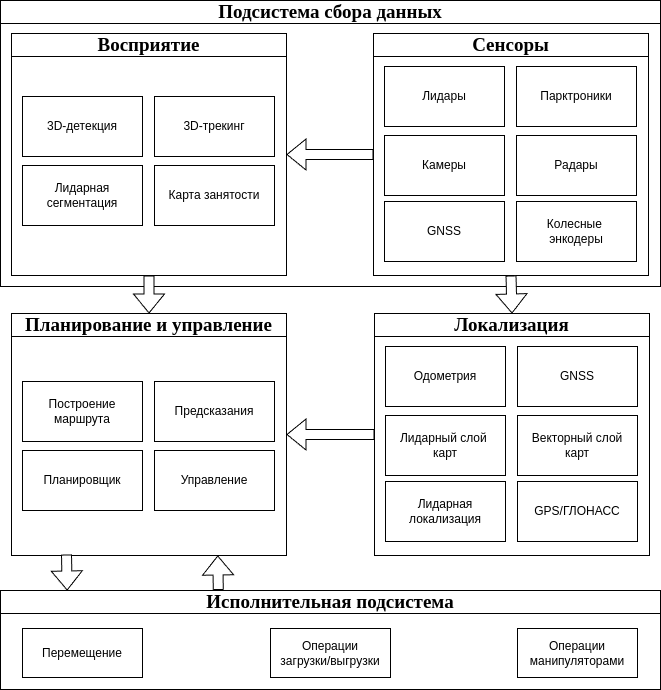
\includegraphics[width=0.95\textwidth]{drawio/arch_tech.drawio.png}
				\vspace*{\fill}
			\end{column}
		\end{columns}
	\end{frame}

	\begin{frame}{Основа для классификации}
		\begin{columns}[onlytextwidth,T]
			% Левая колонка с текстом
			\begin{column}{0.4\textwidth}
				\centering
				\vspace{5em} % Верхний отступ-пружина
				\begin{minipage}[c]{0.95\textwidth} % Ограничиваем ширину для переноса
					\begin{itemize}
						\item ЭМВОС (модель OSI);
						\item модель TCP/IP.
					\end{itemize}
				\end{minipage}
				\vspace*{\fill} % Нижний отступ-пружина
			\end{column}

			% Правая колонка с изображениями
			\begin{column}{0.5\textwidth}
				\centering
				\vspace{2em}
				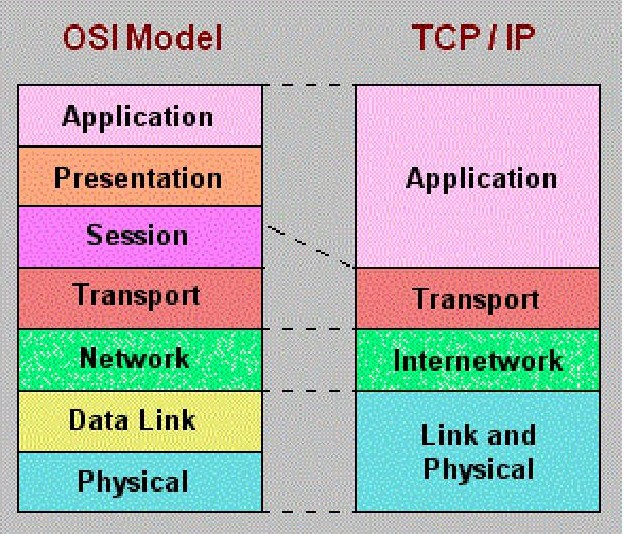
\includegraphics[width=0.9\textwidth]{views/osi.jpg}
				\vspace*{\fill}
			\end{column}
		\end{columns}
	\end{frame}

	\begin{frame}{Среды и~уровни взаимодействия}
		\begin{columns}[onlytextwidth,T]
			% Левая колонка с текстом
			\begin{column}{0.4\textwidth}
				\centering
				\vspace{5em}
				\begin{minipage}[c]{0.95\textwidth} % Ограничиваем ширину для переноса
					\begin{itemize}
						\item физический;
						\item логический.
					\end{itemize}
				\end{minipage}
				\vspace*{\fill} % Нижний отступ-пружина
			\end{column}

			% Правая колонка с изображениями
			\begin{column}{0.5\textwidth}
				\centering
				\vspace{2em}
				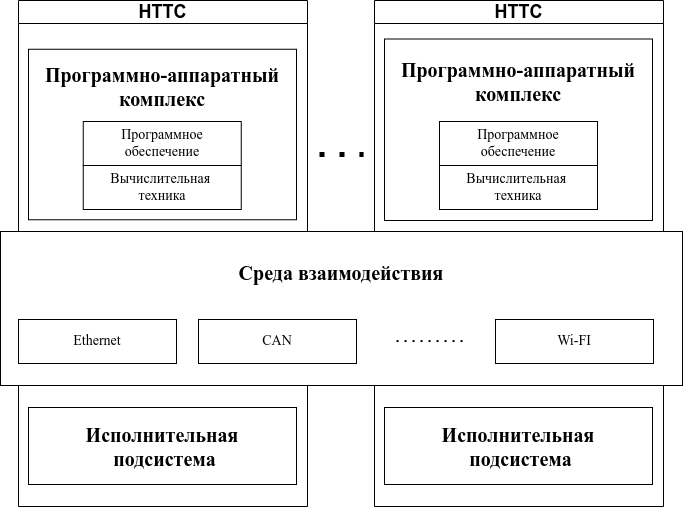
\includegraphics[width=\textwidth]{drawio/po.drawio.png}
				\vspace*{\fill}
			\end{column}
		\end{columns}
	\end{frame}

	\begin{frame}{Внутренняя сеть связи}
		\begin{columns}[T,onlytextwidth]
			\begin{column}{0.4\textwidth}
				\centering
				\vspace*{\fill} % Верхний отступ-пружина
				\begin{minipage}[t][0.5\textheight][c]{\columnwidth} % Ограничиваем ширину для переноса
					\begin{itemize}\setlength\itemsep{3mm}
						\item универсальная последовательная шина;
						\item сеть контроллеров;
						\item проводной Ethernet.
					\end{itemize}
				\end{minipage}
				\vspace*{\fill} % Нижний отступ-пружина
			\end{column}
			\begin{column}{0.5\textwidth}
				\centering
				\vspace{2em}
				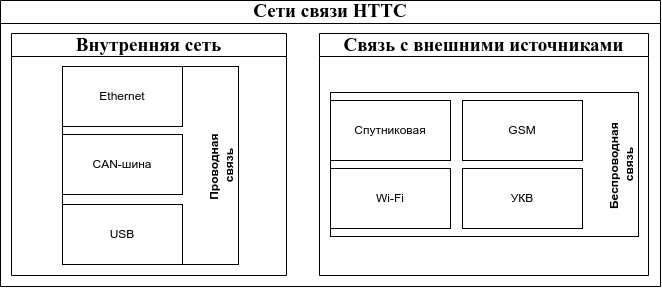
\includegraphics[width=\textwidth]{drawio/ntts_link.drawio.png}
				\vspace*{\fill}
			\end{column}
		\end{columns}
	\end{frame}

	\begin{frame}{Внешняя сеть связи}
		\begin{columns}[T,onlytextwidth]
			\begin{column}{0.4\textwidth}
				\centering
				\vspace*{\fill} % Верхний отступ-пружина
				\begin{minipage}[t][0.5\textheight][c]{\columnwidth} % Ограничиваем ширину для переноса
					\begin{itemize}
						\item сети мобильной связи;
						\item сети спутниковой связи;
						\item Wi-Fi;
						\item УКВ.
					\end{itemize}
				\end{minipage}
				\vspace*{\fill} % Нижний отступ-пружина
			\end{column}
			\begin{column}{0.5\textwidth}
				\centering
				\vspace{2em}
				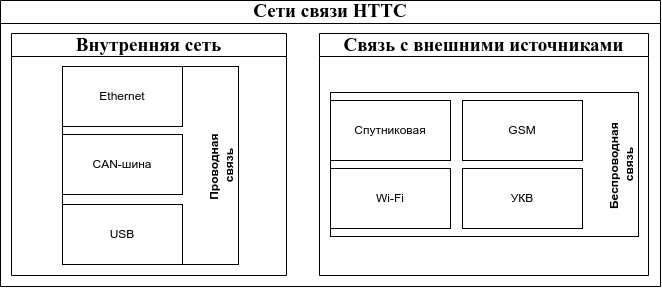
\includegraphics[width=\textwidth]{drawio/ntts_link.drawio.png}
				\vspace*{\fill}
			\end{column}
		\end{columns}
	\end{frame}

	\begin{frame}{Сравнение технологий беспроводной связи}
		\begin{table}[htbp]
			\centering
			\resizebox{\textwidth}{!}{%
				\begin{threeparttable}
					\begin{tabular}{|c|c|c|c|c|c|}
						\hline
						\textbf{Технология} & \textbf{Покрытие} & \textbf{Надежность} & \textbf{Скорость} & \textbf{Задержка} & \textbf{Применение} \\ \hline
						\makecell{4G/5G} & \makecell{Городские\\районы} & Высокая & \makecell{1-10 Гбит/с} & \makecell{1-50 мс} & \makecell{Управление\\в реальном времени} \\ \hline
						\makecell{Спутниковая} & Глобальное & Средняя & \makecell{100-500 Мбит/с} & \makecell{20-800 мс} & \makecell{Удаленные\\районы} \\ \hline
						Wi-Fi & \makecell{Локальное} & Высокая & \makecell{3.5-9.6 Гбит/с} & \makecell{1-20 мс} & \makecell{Локальная связь} \\ \hline
						УКВ & \makecell{До 50 км} & Низкая & \makecell{до 10 Мбит/с} & \makecell{100-500 мс} & \makecell{Резервная связь} \\ \hline
					\end{tabular}
				\end{threeparttable}
			}
		\end{table}
	\end{frame}

	\begin{frame}{Логический уровень}
		\begin{columns}[T,onlytextwidth]
			\begin{column}{0.4\textwidth}
				\vspace{5em} % Верхний отступ-пружина
				Определяет протоколы передачи данных, обеспечивающие надежность и целостность связи. Данные инкапсулируются в кадры физического уровня
				\vspace*{\fill} % Нижний отступ-пружина
			\end{column}
			\begin{column}{0.5\textwidth}
				\vspace{2em}
				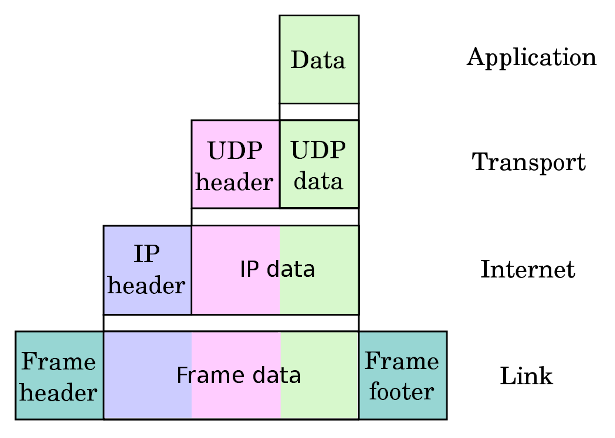
\includegraphics[width=\textwidth]{views/tcp_udp.png}
				\vspace*{\fill}
			\end{column}
		\end{columns}
	\end{frame}

	\begin{frame}{Информационные протоколы}
		\begin{columns}[T,onlytextwidth]
			\begin{column}{0.4\textwidth}
				\centering
				\vspace{4em} % Верхний отступ-пружина
				\begin{minipage}[t][0.4\textheight][c]{\columnwidth} % Ограничиваем ширину для переноса
					\begin{itemize}
						\item протоколы адресования:
						\begin{enumerate}
							\item IP, OSPF, BGP, IS-IS и др.;
							\item единого сетевого (стека) протоколов информационного обмена;
						\end{enumerate}

						\item транспортные протоколы:
						\begin{enumerate}
							\item MQTT;
							\item LoRaWAN;
							\item TCP;
							\item UDP;
							\item QUIC;
							\item MultipathTCP.
						\end{enumerate}
					\end{itemize}
				\end{minipage}
				\vspace*{\fill} % Нижний отступ-пружина
			\end{column}
			\begin{column}{0.5\textwidth}
				\vspace{2em}
				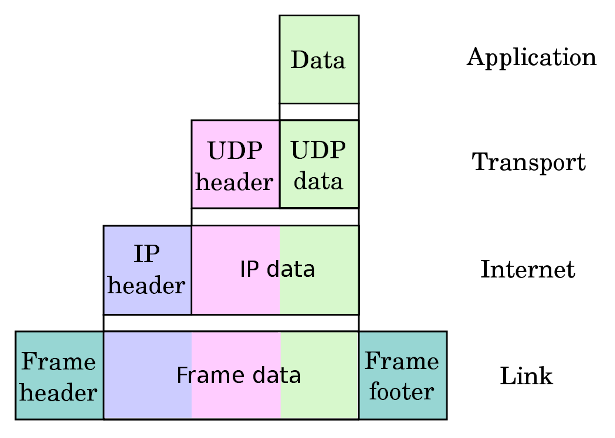
\includegraphics[width=\textwidth]{views/tcp_udp.png}
				\vspace*{\fill}
			\end{column}
		\end{columns}
	\end{frame}

	\begin{frame}{Сравнение протоколов на транспортном уровне}
		 \begin{table}[htbp]
			\centering
			\resizebox{\textwidth}{!}{%
				\begin{threeparttable}
					\begin{tabular}{|l|c|c|c|c|c|c|c|c|}
						\hline
						Протокол & Надежность & \makecell{Эффективность\\ использования\\ канала} & \makecell{Контрольная\\ сумма} & Таймер & \makecell{Подтверждение\\ получения} & \makecell{Отрицательное\\ подтверждение} & Конвейер & Применение \\ \hline
						MQTT & \makecell{Частичная\\ (QoS 0-2)} & Низкая & Нет & Нет & \makecell{Да\\ (QoS \geq 1)} & Нет & Нет & \makecell{IoT-датчики,\\ телеметрия} \\ \hline
						LoRaWAN & Средняя & Низкая & Да & Да & Опция & Нет & Нет & \makecell{Удаленные\\ сенсоры} \\ \hline
						TCP & Высокая & Средняя & Да & Да & Да & Да & Да & \makecell{Веб, передача\\ файлов} \\ \hline
						UDP & Низкая & \textbf{Макс.} & Опц. & Нет & Нет & Нет & Нет & \makecell{Потоковые данные,\\ VoIP} \\ \hline
						QUIC & Высокая & Высокая & Да & Да & Да & Да & Да & \makecell{Мобильные\\ приложения} \\ \hline
						MultipathTCP & \textbf{\makecell{Очень\\ высокая}} & Высокая & Да & Да & Да & Да & Да & \makecell{Критические\\ системы} \\ \hline
					\end{tabular}
				\end{threeparttable}
			}
		\end{table}
	\end{frame}

\end{document}